\chapter*{Abstrakt}
Práce se zabývá principem fungování servomotorů, jejich konstrukcí a možnostmi řízení. Nejprve vysvětluje význam zpětné vazby, jednotlivé způsoby snímání polohy a základní druhy servopohonů. Na modelovém příkladu otočného držáku jsou následně stanoveny požadavky na pohon a vybrán vhodný servomotor MG996R. Dále je popsán princip řízení pomocí PWM signálu a navrženy dvě varianty řídicího obvodu, jedna s časovačem NE555 a druhá s pomocí mikrokontroléru. Součástí práce jsou také zásady návrhu napájení, vedení zemních spojů a omezení elektromagnetického rušení.


\chapter{Teoretická část -- princip servomotoru}
\section{Co je to servo}
Servo je pohon, který umožňuje přesně řídit polohu, rychlost nebo moment osy. Na rozdíl od běžného motoru, který se po přivedení napětí začne otáčet, servo využívá řídicí elektroniku a~zpětnou vazbu. Nejde tedy o konkrétní druh elektromotoru, ale o celý regulační systém.

\section{Zpětná vazba a polohová regulace}
Princip fungování spočívá v~porovnávání požadovaného a skutečného stavu. Servo obsahuje snímač. který průběžně sleduje například natočení hřídele a předává tuto informaci regulátoru. Ten vyhodnotí rozdíl oproti požadované poloze a podle potřeby motor roztočí, zpomalí nebo zastaví. Pokud na hřídel působí vnější síla, regulátor může motor dále napájet, aby požadovanou polohu udržel. Přesnost ovlivňuje kvalita snímače, nastavení regulace i mechanické vůle.

U~modelářských polohových RC serv jsou motor, snímač i řídicí elektronika umístěny v~jednom pouzdře a nadřazený systém pouze zadává požadovanou polohu, což výrazně zjednodušuje celý projekt. Průmyslové servopohony naopak obvykle používají samostatný servozesilovač, který řídí polohu, rychlost a proud motoru. Pro snímání polohy se zde často využívají enkodéry nebo resolvery.~\cite{omron}

\vspace{5mm}

\noindent\begin{minipage}{\textwidth}\centering
\resizebox{.95\textwidth}{!}{\begin{tikzpicture}[font=\footnotesize,x=1cm,y=1cm]
\node[blok,text width=19mm] (p) at (1,2) {Regulátor\\polohy};
\node[blok,text width=19mm] (v) at (4,2) {Regulátor\\rychlosti};
\node[blok,text width=19mm] (i) at (7,2) {Regulátor\\proudu};
\node[blok,text width=22mm] (m) at (10.5,2) {Měnič\\a motor};
\draw[tok] (-1,2)--node[above]{$\varphi^*$}(p);
\draw[tok] (p)--node[above]{$\omega^*$}(v);
\draw[tok] (v)--node[above]{$i^*$}(i);
\draw[tok] (i)--node[above]{buzení}(m);
\draw[tok] (m.south)--(10.5,.8)--node[below]{měřený proud}(7,.8)--(i.south);
\draw[tok,accent] (m.east)--(12.3,2)--(12.3,-.3)--node[below]{rychlost z odměřování}(4,-.3)--(v.south);
\draw[tok,accent] (12.3,-.3)--(12.3,-1.4)--node[below]{poloha z enkodéru / resolveru}(1,-1.4)--(p.south);
\fill[accent] (12.3,-.3) circle(1.5pt);
\end{tikzpicture}
}
\captionsetup{hypcap=false}\captionof{figure}{Kaskádní regulace průmyslového servopohonu.}
\end{minipage}

\section{Snímače zpětné vazby}
Pro zpětnou vazbu je potřeba znát aktuální stav natočení hřídele, případně stav lineárního pohonu. K tomu se používají různé druhy snímaču. V zásadě se dělí na: 
\begin{itemize}
    \item \textbf{Inkrementální}: snímač poskytuje přírůstky polohy; po ztrátě údaje obvykle potřebuje referování. 
    \item \textbf{Absolutní}: snímač určí polohu v~daném rozsahu již po zapnutí.~\cite{heidenEncoders}
\end{itemize}
V praxi se pak používají konkrétní typy senzorů popsané v dalších sekcích. 

\subsection{Potenciometr}
Jezdec spojený s otočnou hřídelí dělí napětí na odporové drážce. Elektronika RC serva, například SG90 či MG996R, porovnává toto napětí se setpointem. Výhodou je nízká cena a jednoduché absolutní měření v~omezeném rozsahu. Nevýhodou je opotřebení kontaktu, šum jezdce a omezený počet otáček.

\subsection{Optický enkodér}
LED svítí přes periodicky s opakující průsvitná okénka v kotouči na fotodetektor a komparátor převádí odezvu na logické úrovně. Optické snímání se používá v~přesných průmyslových odměřováních i lineárních pravítkách. Nabízí vysoké rozlišení a bezkontaktní čtení, vyžaduje však čistou optickou cestu a přesné uložení.~\cite{microchipSensors}

\noindent\begin{minipage}{\textwidth}\centering
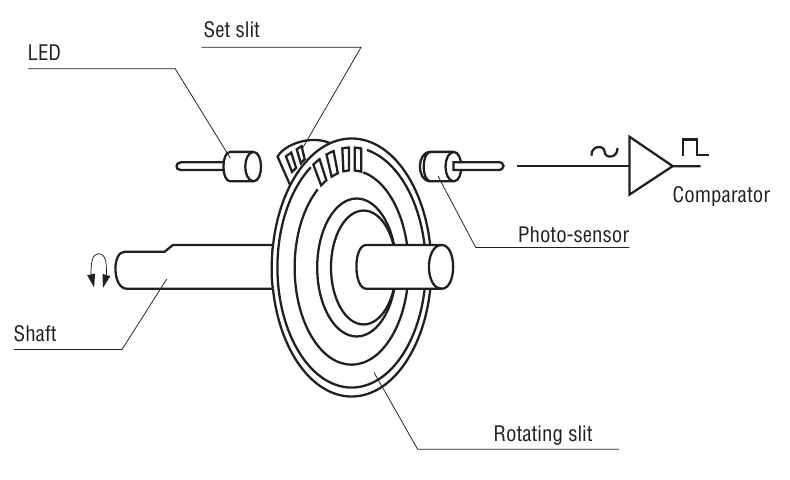
\includegraphics[width=.48\textwidth]{obrazky/foto/opticky-princip.png}
\captionsetup{hypcap=false}\captionof{figure}{LED, dělený kotouč a fotodetektor.~\cite{fotoKotouc}}
\end{minipage}

Často se používají dva výstupní signály A a B, které jsou vzájemně posunuté o čtvrtinu periody. Z jejich pořadí lze určit směr otáčení a počítáním změn signálů zjistit natočení hřídele. Při vyhodnocení všech hran získáme čtyřikrát více kroků než při počítání celých period. Doplňkový signál Z označuje jednu referenční polohu během otáčky.~\cite{microchipQEI}

\vspace{5mm}

\noindent\begin{minipage}{\textwidth}\centering
\resizebox{.95\textwidth}{!}{\begin{tikzpicture}[x=.9cm,y=.8cm]
\foreach \shift/\title in {0/{A předbíhá B},8/{B předbíhá A}} {
 \begin{scope}[xshift=\shift cm]
 \node[font=\small\bfseries] at (2.7,3.2) {\title};
 \node[left] at (0,2.2) {A}; \node[left] at (0,.7) {B};
 \draw[gray!40] (0,1.8)--(5.6,1.8) (0,.3)--(5.6,.3);
 \draw[->] (0,-.35)--(5.8,-.35) node[right] {$t$};
 \ifnum\shift=0
  \def\a{.5}\def\b{1}
 \else
  \def\a{1}\def\b{.5}
 \fi
 \foreach \base/\start in {1.8/\a,.3/\b} {
  \draw[accent,thick] (0,\base)--(\start,\base)
   --(\start,\base+.8)--(\start+1,\base+.8)--(\start+1,\base)
   --(\start+2,\base)--(\start+2,\base+.8)--(\start+3,\base+.8)
   --(\start+3,\base)--(\start+4,\base)--(\start+4,\base+.8)--(5.6,\base+.8);
 }
 \draw[<->] (.5,2.85)--(1,2.85) node[midway,above,font=\scriptsize] {$T/4$};
 \ifnum\shift=0
  \node[below,font=\scriptsize] at (2.8,-.65) {$00\to10\to11\to01\to00$};
 \else
  \node[below,font=\scriptsize] at (2.8,-.65) {$00\to01\to11\to10\to00$};
 \fi
 \end{scope}
}
\node[below,align=center,font=\footnotesize] at (7,-1.3) {Stav je zapsán jako AB. Při vyhodnocení $\times4$ se počítá každá hrana;\\opačné pořadí stavů obrací znaménko přírůstku polohy.};
\end{tikzpicture}
}
\captionsetup{hypcap=false}\captionof{figure}{Kvadraturní signály při opačných směrech pohybu.}
\end{minipage}

\subsection{Magnetický snímač}

Magnetický snímač určuje polohu hřídele podle magnetického pole. Na hřídeli je umístěn magnet, jehož natočení snímá například Hallův senzor, např. dvouosý AS5048. Magnetické snímače se používají především v~robotice a menších pohonech. Jejich výhodou je bezkontaktní měření a~odolnost vůči nečistotám. Nevýhodou je citlivost na přesné umístění magnetu a okolní magnetická pole.~\cite{as5048}


\subsection{Resolver}

Resolver je snímač polohy pracující na principu elektromagnetické indukce, podobně jako transformátor. Střídavý proud v~budicím vinutí vytváří magnetické pole, které indukuje napětí ve dvou snímacích vinutích. Velikost těchto napětí závisí na natočení rotoru, díky čemuž lze určit polohu hřídele. U~klasického resolveru je budicí vinutí na rotoru, zatímco u~reluktančního provedení jsou všechna vinutí na statoru. 

Resolver se používá především v~průmyslových a trakčních pohonech. Jeho výhodou je vysoká mechanická a tepelná odolnost, nevýhodou je potřeba střídavého buzení a složitější vyhodnocovací elektroniky.~\cite{resolverADI}


\noindent\begin{minipage}{\textwidth}\centering
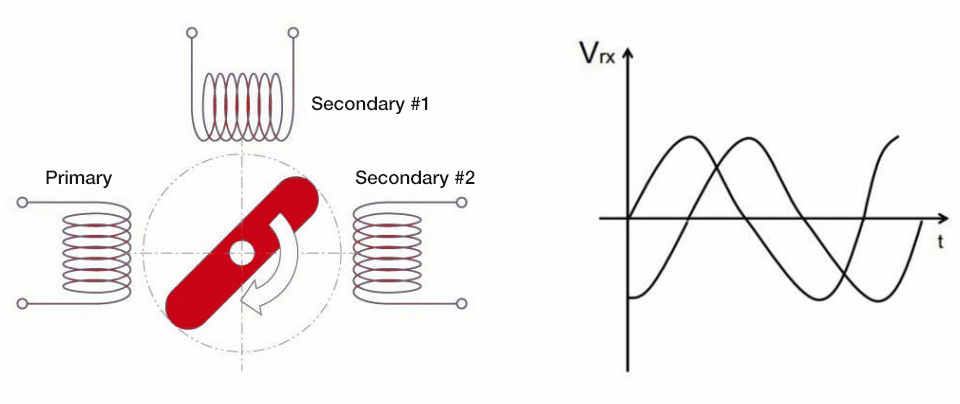
\includegraphics[width=.68\textwidth]{obrazky/foto/resolver-princip.jpg}
\captionsetup{hypcap=false}\captionof{figure}{Princip reluktančního resolveru.~\cite{fotoResolver}}
\end{minipage}

\subsection{Indukční enkodér}

Indukční enkodér, jak již název napovídá, pracuje také na principu elektromagnetické indukce. Střídavý proud v~budicí cívce vytváří magnetické pole, které vyvolává vířivé proudy ve vodivém terči spojeném s~hřídelí. Natočení terče ovlivňuje magnetické pole a tím i napětí indukované ve snímacích cívkách. Z~těchto změn elektronika určuje polohu hřídele. Cívky bývají často vytvořeny přímo na plošném spoji, díky čemuž může být snímač menší a levnější než klasický resolver. Výhodou je bezkontaktní měření a odolnost vůči nečistotám, nevýhodou jsou nároky na přesné umístění terče vůči cívkám a potřeba vyhodnocovací elektroniky.~\cite{tiInductive}


\noindent\begin{minipage}{\textwidth}\centering
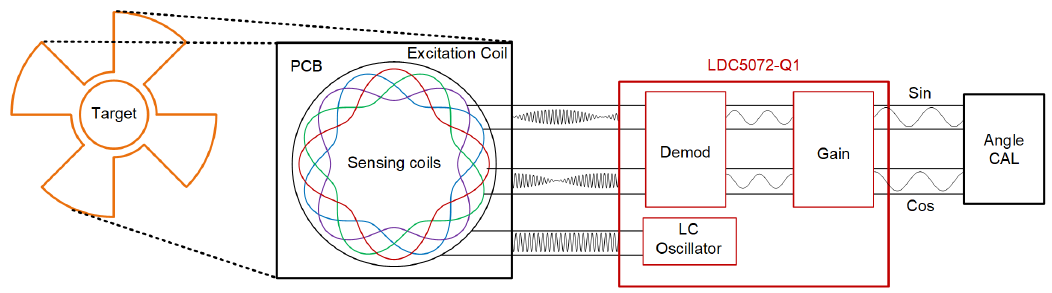
\includegraphics[width=.88\textwidth]{obrazky/foto/indukcni-princip.png}
\captionsetup{hypcap=false}\captionof{figure}{Vodivý terč, plošné cívky a vyhodnocení.~\cite{fotoIndukcni}}
\end{minipage}

\Needspace{75mm}
\section{Druhy servomotorů a jejich konstrukce}
Servomotory se liší konstrukcí, způsobem řízení i oblastí použití. Mezi běžné skupiny patří průmyslové servopohony, lineární servopohony a modelářská serva. V této práci se budeme dále zabývat hlavně těmi.

\Needspace{55mm}
\subsection{Modelářská serva}
\noindent\begin{minipage}{\textwidth}
\begin{minipage}[t]{.61\textwidth}\vspace{0pt}
Modelářská RC serva obsahují malý elektromotor, převodovku a řídicí elektroniku v~jednom pouzdře. Převodovka snižuje otáčky a zvyšuje výstupní moment, zároveň však přináší mechanické vůle. Běžná polohová serva, například SG90 nebo MG996R, mají navíc snímač polohy a nastavují a udržují požadovaný úhel, často v~rozsahu přibližně 180°. 

Kontinuální serva, například FS90R, umožňují nepřetržité otáčení, přičemž řídicí pulzy PWM určují směr a přibližnou rychlost místo polohy. Používají se v~modelářství, robotice a~jednoduchých mechanismech.
\end{minipage}\hfill
\begin{minipage}[t]{.35\textwidth}\vspace{0pt}\centering
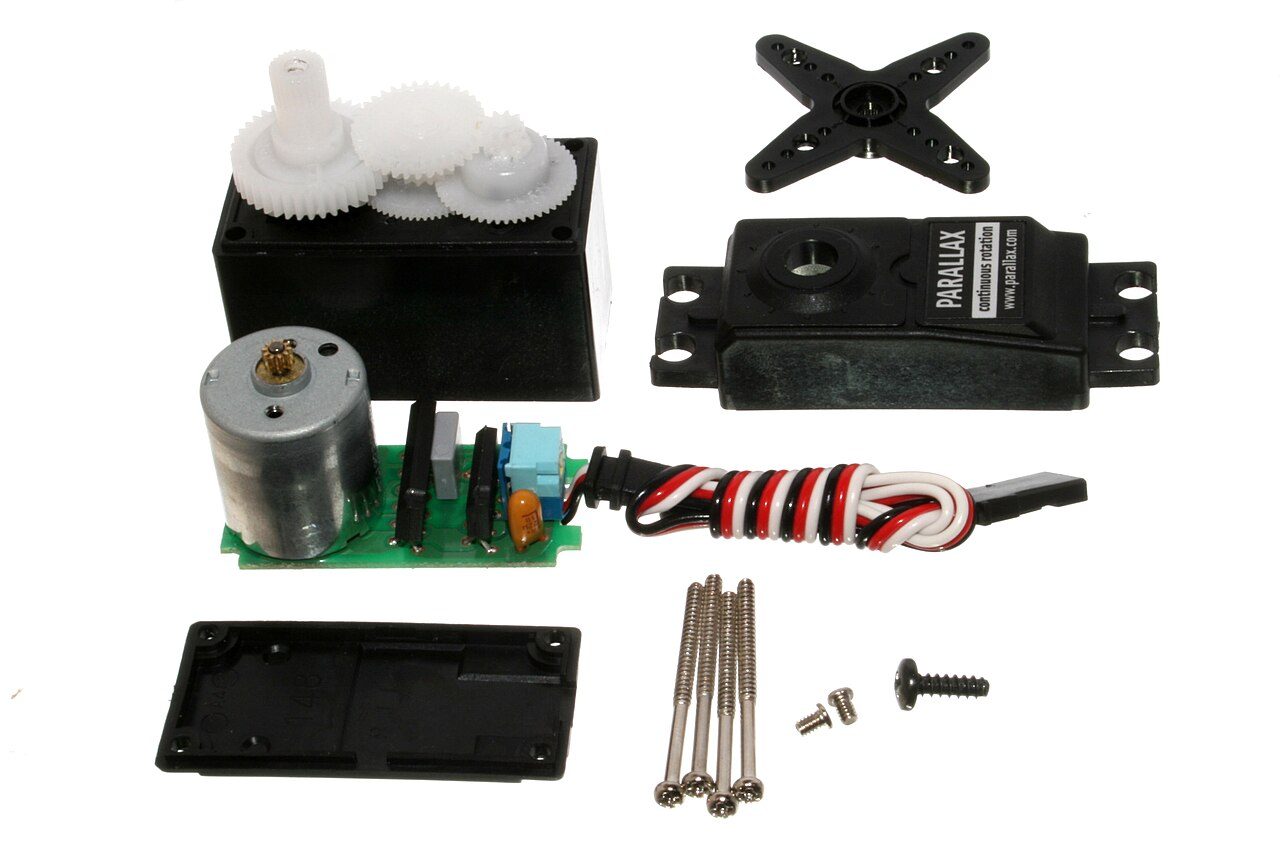
\includegraphics[width=\linewidth,height=30mm,keepaspectratio]{obrazky/foto/rozebrane-servo.jpg}
\captionsetup{hypcap=false,justification=raggedright,singlelinecheck=false}\captionof{figure}{Vnitřek RC serva.~\cite{fotoRozebrane}}
\end{minipage}
\end{minipage}\par

\Needspace{55mm}
\subsection{Průmyslové servopohony}
\noindent\begin{minipage}{\textwidth}
\begin{minipage}[t]{.61\textwidth}\vspace{0pt}
Průmyslové servopohony se používají tam, kde je potřeba vysoká přesnost, výkon a spolehlivost. Často využívají bezkartáčové synchronní motory s~permanentními magnety, případně asynchronní motory se zpětnovazebním řízením. Polohu snímá enkodér nebo resolver a chod motoru řídí servozesilovač. Umožňují přesné řízení polohy, rychlosti i~momentu a používají se například v~průmyslových robotech, CNC strojích a automatizovaných výrobních linkách.~\cite{omron}
\end{minipage}\hfill
\begin{minipage}[t]{.35\textwidth}\vspace{0pt}\centering
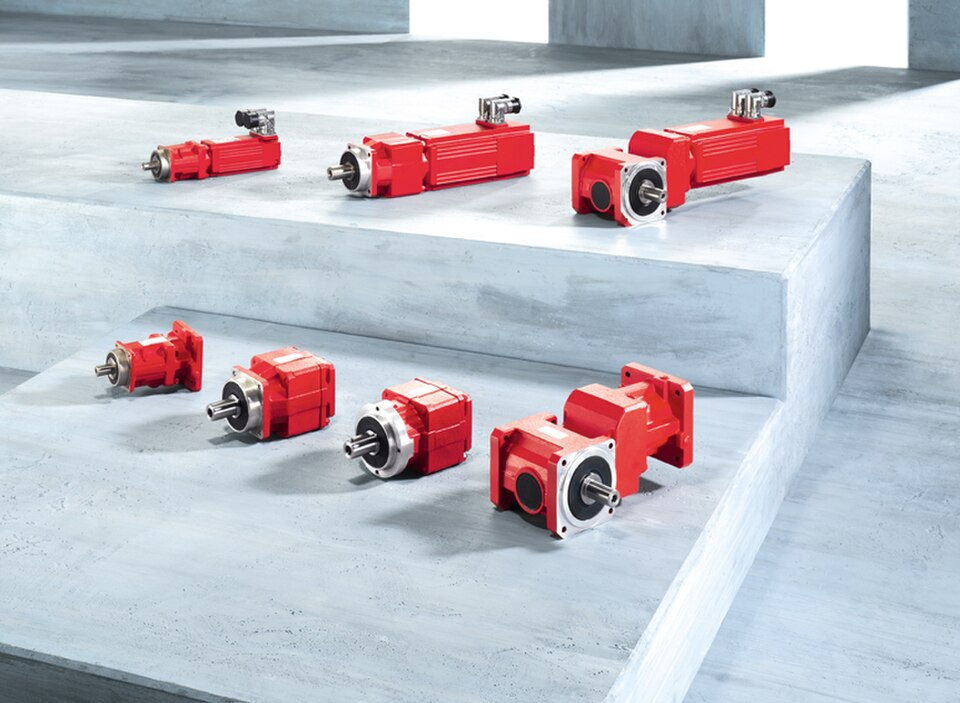
\includegraphics[width=\linewidth,height=30mm,keepaspectratio]{obrazky/foto/prumyslove-pohony.jpg}
\captionsetup{hypcap=false,justification=raggedright,singlelinecheck=false}\captionof{figure}{Průmyslové pohony.~\cite{fotoPrumysl}}
\end{minipage}
\end{minipage}\par

\vspace{5mm}
\noindent\begin{minipage}{.54\textwidth}
Snímač v tomto servu bývá umístěn na zadním konci hřídele. Jeho otočná část sleduje rotor, pevná část předává údaj zesilovači. Vůli převodovky za motorem takové měření přímo nezachytí. Přesnější osy mohou mít další snímač na výstupu nebo lineární pravítko, kterým se sleduje až výsledný efekt posunu na ose.~\cite{heidenRobot}

\end{minipage}\hfill
\begin{minipage}{.42\textwidth}\centering
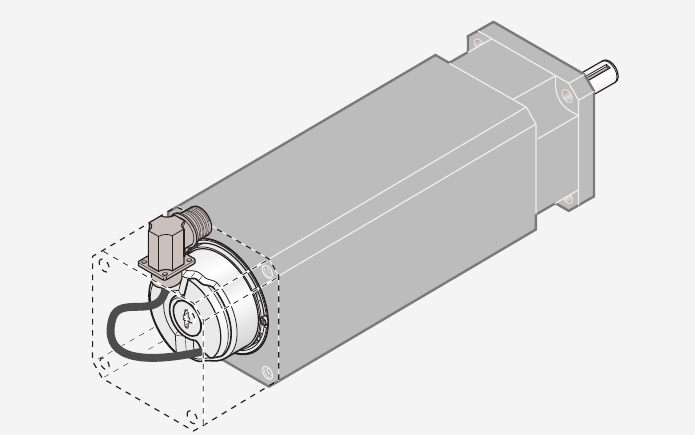
\includegraphics[width=\linewidth,height=35mm,keepaspectratio]{obrazky/foto/motor-odmerovani.png}
\captionsetup{hypcap=false}\captionof{figure}{Snímač v~motoru.~\cite{fotoMotorOdmerovani}}
\end{minipage}

\Needspace{55mm}
\subsection{Lineární servopohony}
\noindent\begin{minipage}{\textwidth}
\begin{minipage}[t]{.61\textwidth}\vspace{0pt}
Lineární servopohony slouží k~přesnému řízení přímočarého pohybu namísto otáčení. Mohou využívat přímo lineární elektromotor nebo běžný rotační servomotor, jehož pohyb se převádí například kuličkovým šroubem či řemenem na posuv. Zpětná vazba umožňuje přesně řídit polohu a rychlost pohybu, případně i sílu. Uplatňují se především v~automatizaci, polohovacích systémech a posuvových osách obráběcích strojů.
\end{minipage}\hfill
\begin{minipage}[t]{.35\textwidth}\vspace{0pt}\centering
% Dočasný obrázek; nahradit fotografií lineárního servopohonu.
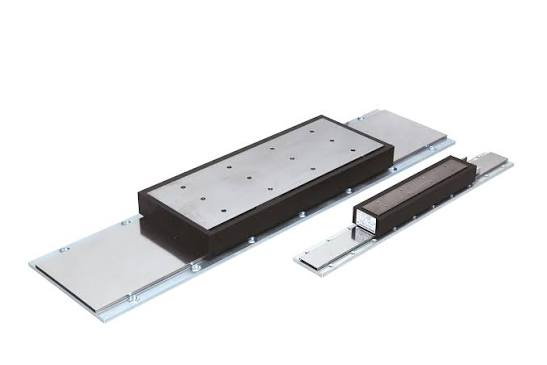
\includegraphics[width=\linewidth,height=30mm,keepaspectratio]{obrazky/foto/linear_servo.jpeg}
\captionsetup{hypcap=false,justification=raggedright,singlelinecheck=false}\captionof{figure}{Lineární servo od Yaskawa.~\cite{fotoLinear}}
\end{minipage}
\end{minipage}\par